\documentclass[a4paper]{article}

\usepackage{polski}
\usepackage[utf8]{inputenc}

\usepackage{scrextend}
\usepackage{amsfonts}
\usepackage{amsmath}
\usepackage{svg}

\usepackage{geometry}
\geometry{a4paper, left=15mm, top=30mm, right=15mm}

\usepackage{graphicx} 
\usepackage{isotope}
\usepackage{array}

\usepackage{hyperref}
\hypersetup{
    colorlinks,
    citecolor=black,
    filecolor=black,
    linkcolor=black,
    urlcolor=black
}

\date{}

\newenvironment{definition}[1][title]
    {
        \begin{center}
        \begin{tabular}{|p{1\textwidth}|}
        \hline\\
            Definicja: #1\\[2ex]
        \begin{em}
        \Large
    }
    { 
        \end{em}
        \\\\\hline
        \end{tabular} 
        \end{center}
    }
    
\begin{document}
    \linespread{1.5}
    \begin{titlepage}
        \centering
        \vspace*{\fill}

        \vspace*{0.5cm}

        \huge\bfseries
        Notatki z wykładów z Fizyki 1

        \vspace*{0.5cm}

        \large Łukasz Kwinta

        \vspace*{\fill}
    \end{titlepage}
    
\pagebreak
\tableofcontents
\pagebreak

\section{\huge Wiadomości wstępne i wektory}
    \subsection{\LARGE Suma wektorów}
        \Large 
        Niech:
        \[\vec{a} := (a_1, a_2, a_3) \hspace{1cm} \vec{b} = (b_1, b_2, b_3) \]
        Wtedy suma wektorów ma następującą postać:
        \[\vec{a} + \vec{b} = (a_1 + b_1,\ a_2 + b_2,\ a_3 + b_3)\] \\
        \begin{center}
            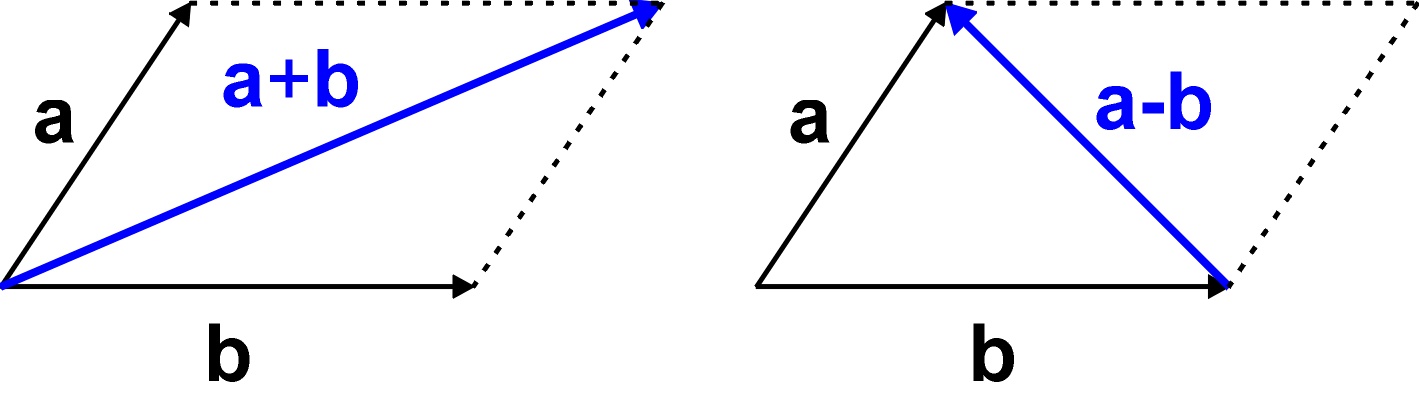
\includegraphics[width=10cm]{suma_wektorow.png} 
        \end{center}
        
    \subsection{\LARGE Iloczyn skalarny}
        \Large 
        Niech:
        \[\vec{a} := (a_1, a_2, a_3) \hspace{1cm} \vec{b} = (b_1, b_2, b_3) \]
        Wtedy iloczyn skalarny oznaczamy $\circ$ ma następującą postać:
        \[\vec{a} \circ \vec{b} = a_1 \cdot b_1 + a_2 \cdot b_2 + a_3 \cdot b_3\]
        Występuje również poniższa zależność:
         \[\vec{a} \circ \vec{b} = ||\vec{a}|| \cdot ||\vec{b}|| \cdot \cos{(\ \vec{a},\ {\vec{b}}\ )} \]
        
    \subsection{\LARGE Iloczyn wektorowy}
        \Large 
        Niech:
        \[\vec{a} := (a_1, a_2, a_3) \hspace{1cm} \vec{b} = (b_1, b_2, b_3) \]
        oraz:      
        \[\vec{i} := (1, 0, 0) \hspace{0,75cm} \vec{j} = (0, 1, 0) \hspace{0,75cm} \vec{k} = (0, 0, 1) \]
        Wtedy, iloczyn wektorowy ma następującą postać:
        \[
            \vec{a} \times \vec{b} = 
            \begin{vmatrix}
                \vec{i} & \vec{j} & \vec{k} \\
                a_1 & a_2 & a_3 \\
                b_1 & b_2 & b_3
            \end{vmatrix}
            = \vec{i}(a_2b_3 - a_3b_2) + \vec{j}(a_3b_1 - a_1b3) + \vec{k}(a_1b_2 - a_2b_1) =     
        \]
        \[ = (a_2b_3 - a_3b_2, a_3b_1 - a_1b3, a_1b_2 - a_2b_1 )\]
        Tak jak przy iloczynie skalarnym występuje zależność związana z kątem między wektorami:
        \[||\vec{a} \times \vec{b}|| = ||\vec{a}||\cdot ||\vec{b}|| \cdot \sin{(\ \vec{a},\ {\vec{b}}\ )}\]
        Kierunek iloczynu wektorowego $\vec{a} \times \vec{b}$ jest prostopadły do płaszczyzny 
        stworzonej przez wektory $\vec{a}$ i $\vec{b}$.\\ Natomiast zwrot tego wektora można określić stosując zasadę prawej dłoni: \\
        \begin{center}
            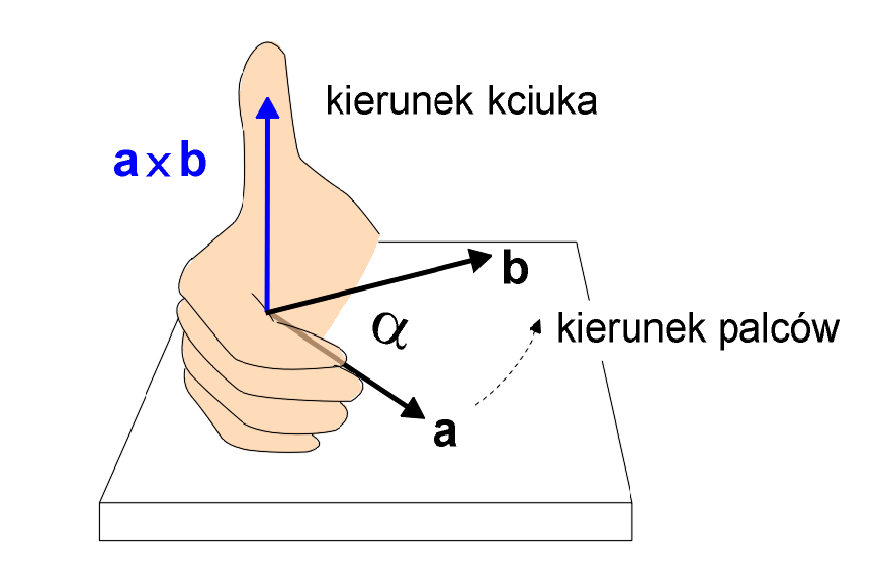
\includegraphics[width=15cm]{prawareka.png} 
        \end{center}
        
\section{\huge Podstawy kinematyki}
    \subsection{\LARGE Podstawowe pojęcia}
        \begin{definition}[Ruch]
            Zmiana wzajemnego położenia ciał względem innych ciał wraz z upływem czasu.
        \end{definition}
        \begin{definition}[Układ odniesienia]
            Wybrane ciało lub ciało względem których wyznaczamy własności fizyczne takie jak położenie czy prędkość.
        \end{definition}
        \begin{definition}[Punkt materialny]
            Punktem materialnym nazywamy obiekt obdarzony masą, których rozmiar (aka objętość) można zaniedbać.
        \end{definition}
    \subsection{\LARGE Prędkość}
        \begin{definition}[Prędkość]
            Zmiana położenia w czasie:
            $\vec{v} = \frac{\Delta\vec{x}}{\Delta t}$
        \end{definition}
        Jeśli ciało znajdowało się w chwili $t_0$ w punkcie $x_0$, a w chwili $t$ w punkcie $x$ to:
        \[x - x_0 = v(t - t_0) \]
        Stąd ($\Delta x := x - x_0$ oraz $\Delta t := t - t_0$):
        \[v = \frac{x - x_0}{t - t_0} = \frac{\Delta x}{\Delta t}\]
        
        Z definicji prędkość jest wielkością wektorową więc warto zwracać uwagę w zadaniach na oznaczenia. W zadaniach gdzie wektor prędkości nie ma stałego kierunku rozważa się składowe wektora prędkości dla uproszczenia zadania - na przykład przy rzucie ukośnym rozważa się składową pionową i poziomą prędkości.\\

        Gdy wartość prędkości zmienia się w czasie nie możemy mówić 
        

\end{document}